\documentclass{article}

\usepackage{graphicx} % Required for inserting images

\setlength{\parindent}{0pt}


\title{Informe de Física}
\author{Paola Russo}
\date{November 2024}




\begin{document}

\maketitle


\section{Introducción}

La densidad es una magnitud que expresa la relación entre la masa y el volumen de un cuerpo. Se puede definir como la cantidad de masa (m) contenida en un determinado volumen (V), Ec. (\ref{eq:def_densidad}).

\begin{equation}
    \rho = \frac{m}{V}
    \label{eq:def_densidad}
\end{equation}

Diversos experimetos han demostrado ser útiles a la hora de fijar conocimientos sobre la densidad en estudiantes de física inicial \cite{Torres_2018}.\\

El objetivo de este trabajo es realizar una experiencia práctica en el aula para observar la diferencia de densidades en distintos fluidos.

\section{Metodología}

Se parte de una muestra de 90 alumnos de 2$^{\circ}$ año de escuela separados en 3 grupos.\\

La metodología de trabajo consiste en los siguientes pasos:
\begin{enumerate}
    \item Para comenzar se calcula la densidad de cada uno de los fluidos: alcool, aceite, agua coloreada, jabón y miel, en una botella de plástico. A partir de esto se infiere qué fluido se posicionará en qué región de la botella.
    \item Luego se colocan los fluidos cuidadosamente dentro de la botella, se observa y se toma una fotografía. A partir de esto se comprueba si es correcto que los fluidos con menos densidad se posicionan arriba y los de mayor densidad abajo.
    \item A continuación se aplica una evaluación del tema.
\end{enumerate}

La Figura \ref{fig:botella} muestra cómo se debe ver el experimento. La discusión planificada incluye por qué los fluidos se separan de esta manera, terminología apropiada, planteo y verificación de hipótesis, y desarrollo de conclusiones por los niños. 
\begin{figure}[ht]
    \centering    
\includegraphics[width=0.6\linewidth]{exp_torre_de_liquidosjpg.jpg}
    \caption{Torre de líquidos.}
    \label{fig:botella}
\end{figure}



\section{Resultados}

La práctica devolvió resultados favorables con respecto al aprendizaje y la incorporación de los conocimientos sobre el tema. Los mismos se muestran en la Tabla \ref{tab:resultados} y Figura \ref{fig:evaluacion}.\\

Los indicadores de la evaluación muestran que el 96\% de los estudiantes comprendión el concepto de la densidad correctamente.\\

\begin{table}[ht]
    \centering
    \begin{tabular}{|c|c|}
    \hline
         & Número de estudiantes \\
         \hline
        Adquirió conocimientos & 86 \\
        No adquirió conocimientos & 4 \\
        Quiere hacer otros experimentos & 90 \\
        \hline
    \end{tabular}
    \caption{Resultados de la evaluación.}
    \label{tab:resultados}
\end{table}

\begin{figure}[ht]
    \centering
    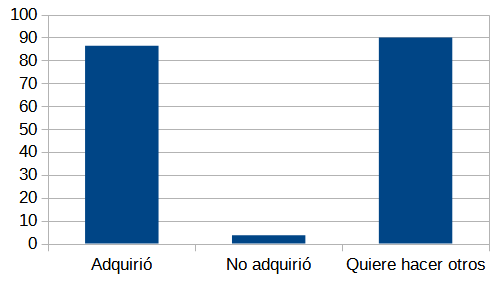
\includegraphics[width=0.6\linewidth]{Grafica.png}
    \caption{Resultados de la evaluación.}
    \label{fig:evaluacion}
\end{figure}


Además, el 100\% de los estudiantes se mostró motivado a continuar realizando experimentos de física.



\section{Conclusiones}

En este trabajo se realizó un breve experimento de física en el aula a nivel de estudiantes de escuela. El experimento consistió en incorporar el concepto de densidad de fluidos.\\

El trabajo logró captar la atención de los estudiantes con una aplicación de uso cotidiano, y motivarlos a continuar experimentando con física en el futuro.





\newpage
\textbf{Disclaimer:} este no es un informe de una experiencia realizada realmente, es sólo un ejemplo inventado a los efectos ilustrativos de cómo escribir un informe.\\

\bibliographystyle{apalike}
\bibliography{main.bib}


\end{document}
